\documentclass[twoside]{article}

% file's preambule


% connect packages
%%%%%%%%%%%%%%%%%%%%%%%%%%%%%%%%%%%%%%%%%%%%%%%%%%%%%%%%%%%%%%%%%%%%%%
\usepackage[T2A]{fontenc}                   %!? закрепляет внутреннюю кодировку LaTeX
\usepackage[utf8]{inputenc}                 %!  закрепляет кодировку utf8
\usepackage[english,russian]{babel}         %!  подключает русский и английский
\usepackage{amsmath}                        %!  |
\usepackage{amssymb,textcomp, esvect,esint} %!  |важно для формул 
\usepackage[margin=2cm]{geometry}           %!  фиксирует оступ на 2cm
\usepackage{amsfonts}                       %!  математические шрифты
\usepackage{amsthm}                         %!  newtheorem и их сквозная нумерация
\usepackage{graphicx}                       %?  графическое изменение текста
\usepackage{indentfirst}                    %   добавить indent перед первым параграфом
\usepackage{xcolor}                         %   добавляет цвета
\usepackage{enumitem}                       %!  задание макета перечня.
\usepackage[unicode, pdftex]{hyperref}      %!  оглавление для панели навигации по PDF-документу + гиперссылки
\usepackage{booktabs}                       %!  добавляет книжные линии в таблицы
\usepackage{hypcap}                         %?  адресация на картинку, а не на подпись к ней
\usepackage{abraces}                        %?  фигурные скобки сверху или снизу текста
\usepackage{caption}                        %-  позволяет корректировать caption 
\usepackage{multirow}                       %   объединение ячеек в таблицах
\usepackage{pifont}                         %!  нужен для крестика
\usepackage{cancel}                         %!  аутентичное перечеркивание текста
\usepackage{ulem}                           %!  перечеркивание текста
\usepackage{tikz}                           %!  высокоуровневые рисунки (кружочек)
\usepackage{titling}                        %-  автоматическое заглавие 
\usepackage{blindtext}                      %-  слепой текст
\usepackage{fancyhdr}                       %   добавить верхний и нижний колонтитул

\usepackage{import}
\usepackage{xifthen}
\usepackage{pdfpages}
\usepackage{transparent}

\usepackage{mathrsfs}  
%%%%%%%%%%%%%%%%%%%%%%%%%%%%%%%%%%%%%%%%%%%%%%%%%%%%%%%%%%%%%%%%%%%%%%

%%%%%%%%%%%%%%%%%%%%%%% ИНТЕГРАЛЫ %%%%%%%%%%%%%%%%%%%%%%%%%%%%%%%%%%%%
\makeatletter
\def\upintkern@{\mkern-7mu\mathchoice{\mkern-3.5mu}{}{}{}}
\def\upintdots@{\mathchoice{\mkern-4mu\@cdots\mkern-4mu}%
 {{\cdotp}\mkern1.5mu{\cdotp}\mkern1.5mu{\cdotp}}%
 {{\cdotp}\mkern1mu{\cdotp}\mkern1mu{\cdotp}}%
 {{\cdotp}\mkern1mu{\cdotp}\mkern1mu{\cdotp}}}
\newcommand{\upiint}{\DOTSI\protect\UpMultiIntegral{2}}
\newcommand{\upiiint}{\DOTSI\protect\UpMultiIntegral{3}}
\newcommand{\upiiiint}{\DOTSI\protect\UpMultiIntegral{4}}
\newcommand{\upidotsint}{\DOTSI\protect\UpMultiIntegral{0}}
\newcommand{\UpMultiIntegral}[1]{%
  \edef\ints@c{\noexpand\upintop
    \ifnum#1=\z@\noexpand\upintdots@\else\noexpand\upintkern@\fi
    \ifnum#1>\tw@\noexpand\upintop\noexpand\upintkern@\fi
    \ifnum#1>\thr@@\noexpand\upintop\noexpand\upintkern@\fi
    \noexpand\upintop
    \noexpand\ilimits@
  }%
  \futurelet\@let@token\ints@a
}
\makeatother

\DeclareFontFamily{OMX}{mdbch}{}
\DeclareFontShape{OMX}{mdbch}{m}{n}{ <->s * [0.8]  mdbchr7v }{}
\DeclareFontShape{OMX}{mdbch}{b}{n}{ <->s * [0.8]  mdbchb7v }{}
\DeclareFontShape{OMX}{mdbch}{bx}{n}{<->ssub * mdbch/b/n}{}

\DeclareSymbolFont{uplargesymbols}{OMX}{mdbch}{m}{n}
\SetSymbolFont{uplargesymbols}{bold}{OMX}{mdbch}{b}{n}
\DeclareMathSymbol{\upintop}{\mathop}{uplargesymbols}{82}
\DeclareMathSymbol{\upointop}{\mathop}{uplargesymbols}{"49}

\DeclareFontEncoding{MDB}{}{}
\DeclareFontFamily{MDB}{mdbch}{}
\DeclareFontShape{MDB}{mdbch}{m}{n}{ <->s * [0.8]  mdbchrmb }{}
\DeclareFontShape{MDB}{mdbch}{b}{n}{ <->s * [0.8]  mdbchbmb }{}
\DeclareFontShape{MDB}{mdbch}{bx}{n}{<->ssub * mdbch/b/n}{}
\DeclareFontSubstitution{MDB}{cmr}{m}{n}
\DeclareSymbolFont{mathdesignB}{MDB}{mdbch}{m}{n}%
\SetSymbolFont{mathdesignB}{bold}{MDB}{mdbch}{b}{n}%
\DeclareMathSymbol{\upintclockwise}{\mathop}{mathdesignB}{128}
\DeclareMathSymbol{\upointclockwise}{\mathop}{mathdesignB}{130}
\DeclareMathSymbol{\upointctrclockwise}{\mathop}{mathdesignB}{132}
\DeclareMathSymbol{\upoiint}{\mathop}{mathdesignB}{134}
\DeclareMathSymbol{\upoiiint}{\mathop}{mathdesignB}{136}

\makeatletter
\newcommand{\upint}{\DOTSI\upintop\ilimits@}
\newcommand{\upoint}{\DOTSI\upointop\ilimits@}
\makeatother

%%%%%%%%%%%%%%%%%%%%%%%%%%%%%%%%%%%%%%%%%%%%%%%%%%%%%%%%%%%%%%%%%%%%%%



% add (renew) commands
%%%%%%%%%%%%%%%%%%%%%%%%%%%%%%%%%%%%%%%%%%%%%%%%%%%%%%%%%%%%%%%%%%%%%%
\renewcommand{\Im}{\mathop{\mathrm{Im}}\nolimits}
\renewcommand{\Re}{\mathop{\mathrm{Re}}\nolimits}
\renewcommand{\div}{\mathop{\mathrm{div}}\nolimits}
\renewcommand{\d}{\, d}
\renewcommand{\leq}{\leqslant}
\renewcommand{\geq}{\geqslant}

\newcommand{\vc}[1]{\mbox{\boldmath $#1$}}
\newcommand{\T}{^{\text{T}}}

\newcommand{\grad}{\mathop{\mathrm{grad}}\nolimits}
\newcommand{\rot}{\mathop{\mathrm{rot}}\nolimits}
\newcommand{\diag}{\mathop{\mathrm{diag}}\nolimits}
\newcommand{\Ker}{\mathop{\mathrm{Ker}}\nolimits}
\newcommand{\Spec}{\mathop{\mathrm{Spec}}\nolimits}
\newcommand{\sign}{\mathop{\mathrm{sign}}\nolimits}
\newcommand{\tr}{\mathop{\mathrm{tr}}\nolimits}
\newcommand{\rg}{\mathop{\mathrm{rg}}\nolimits}

\newcommand{\const}{\text{const}}
\newcommand{\red}[1]{\textcolor{red}{#1}}
\newcommand{\xmark}{\ding{55}}

\renewcommand{\int}{\upint}
\renewcommand{\oint}{\upoint}
%%%%%%%%%%%%%%%%%%%%%%%%%%%%%%%%%%%%%%%%%%%%%%%%%%%%%%%%%%%%%%%%%%%%%%


% some tikz commands
%%%%%%%%%%%%%%%%%%%%%%%%%%%%%%%%%%%%%%%%%%%%%%%%%%%%%%%%%%%%%%%%%%%%%%
\makeatletter %%%%%%%%%%%%%%% КРУЖОЧЕК %%%%%%%%%%%%%%%%%%%%%%%%%%%%%%%
\newcommand*{\encircled}[1]{\relax\ifmmode\mathpalette
\@encircled@math{#1}\else\@encircled{#1}\fi}
\newcommand*{\@encircled@math}[2]{\@encircled{$\m@th#1#2$}}
\newcommand*{\@encircled}[1]{%
  \tikz[baseline,anchor=base]{\node[draw,circle,outer sep=0pt,
                                        inner sep=.2ex] {#1};}}
\makeatother

\usepackage{arydshln} %%%%%%%%%%%%%%% ЛИНИИ В МАТРИЧКЕ %%%%%%%%%%%%%%%
\makeatletter
  \renewcommand*\env@matrix[1][*\c@MaxMatrixCols c]{%
    \hskip -\arraycolsep
    \let\@ifnextchar\new@ifnextchar
  \array{#1}}
\makeatother
%%%%%%%%%%%%%%%%%%%%%%%%%%%%%%%%%%%%%%%%%%%%%%%%%%%%%%%%%%%%%%%%%%%%%%



\DeclareRobustCommand{\tmpsim}{ %%%%%%%%%%%%%% ~ < %%%%%%%%%%%%%%%%%%%
  \mathbin{\text{
      \raisebox{-1pt}{
            \hspace{-4.5pt} \rotatebox{-26}{\scalebox{0.8}[0.7]{$\sim$}}
        }
  }}
}
\def\lesim{{
    \setbox0\hbox{$\ <\ $}
    \rlap{\hbox to \wd0{\hss$\tmpsim$\hss}}\box0
}}
%%%%%%%%%%%%%%%%%%%%%%%%%%%%%%%%%%%%%%%%%%%%%%%%%%%%%%%%%%%%%%%%%%%%%%


% create environment
%%%%%%%%%%%%%%%%%%%%%%%%%%%%%%%%%%%%%%%%%%%%%%%%%%%%%%%%%%%%%%%%%%%%%%
\newtheorem{to_thr}{Thr}[section]
\newtheorem{to_suj}[to_thr]{Suj}
\newtheorem{to_lem}[to_thr]{Lem}
\newtheorem{to_law}[to_thr]{Law}
\newtheorem{to_com}[to_thr]{Com}
\newtheorem{to_con}[to_thr]{Con}
\theoremstyle{definition}
\newtheorem{to_def}[to_thr]{Def}

\newenvironment{description*}
{
    \begin{description}
        \setlength{\itemsep}{1pt}
        \setlength{\parskip}{1pt}
        }
    {\end{description}
}
%%%%%%%%%%%%%%%%%%%%%%%%%%%%%%%%%%%%%%%%%%%%%%%%%%%%%%%%%%%%%%%%%%%%%%

\newcommand{\incfig}[1]{%
    % \def\svgwidth{\columnwidth}
    \import{./figures/}{#1.pdf_tex}
}

% add some colors
%%%%%%%%%%%%%%%%%%%%%%%%%%%%%%%%%%%%%%%%%%%%%%%%%%%%%%%%%%%%%%%%%%%%%%
\definecolor{grey}{HTML}{666666}
\definecolor{linkcolor}{HTML}{0000CC}
\definecolor{urlcolor}{HTML}{006600}
\hypersetup{
    pdfstartview=FitH,  
    linkcolor=linkcolor,
    urlcolor=urlcolor, 
    colorlinks=true,
    citecolor=blue}
%%%%%%%%%%%%%%%%%%%%%%%%%%%%%%%%%%%%%%%%%%%%%%%%%%%%%%%%%%%%%%%%%%%%%%


% add page header
%%%%%%%%%%%%%%%%%%%%%%%%%%%%%%%%%%%%%%%%%%%%%%%%%%%%%%%%%%%%%%%%%%%%%%
\pagestyle{fancy}
\fancyhf{}
\fancyhead[RE,LO]{\textsc{Ф\raisebox{-1.5pt}{и}з\TeX}}
% \fancyhead[LE,RO]{ОбщеФиз}
\fancyhead[CO,CE]{\leftmark}
\fancyfoot[LE,RO]{\textcolor{grey}{\texttt{\thepage}}}
%%%%%%%%%%%%%%%%%%%%%%%%%%%%%%%%%%%%%%%%%%%%%%%%%%%%%%%%%%%%%%%%%%%%%%


\begin{document}

% set skip of equation length 

\setlength{\abovedisplayskip}{3pt}
\setlength{\abovedisplayshortskip}{3pt}
\setlength{\belowdisplayskip}{3pt}
\setlength{\belowdisplayshortskip}{3pt}

% \numberwithin{equation}{section}

% input files


\section*{Articles used}

\begin{enumerate}[label = \Roman*.]
	\item <<Dynamics of Gliding Arc Climbing
in a Unipolar Jacob’s Ladder>> by K. I. Almazov et al. 22 January 2020;

	\item <<Physical study of a gliding arc discharge>> by F. Richard et al. 20 November 1995;

	\item <<Prospects of airflow control by a gliding arc in a static magnetic field>> by N Balcon et al. 28 August 2008;

	\item <<Numerical Calculations of the Properties of Axially Symmetric Arc Columns>> by A.Wells March 1967.
\end{enumerate}
% %%%%%%%%%%%%%%%%%%%%%%%%%%%%%%%%%%%%%%%%%%%%%%%%%%%%%%%%%%%%%%%%%%%%%%%%%%%%
% \section{Principal variables and constants}
% %%%%%%%%%%%%%%%%%%%%%%%%%%%%%%%%%%%%%%%%%%%%%%%%%%%%%%%%%%%%%%%%%%%%%%%%%%%%


% The heat flux potential (потенциал теплового потока) -- 

% The Prandtl and turbulent Prandtl numbers -- 

% The eddy diffusivity for momentum (вихревой коэффициент диффузии для импульса) -- 

% The specific enthalpy (удельная энтальпия) --



%%%%%%%%%%%%%%%%%%%%%%%%%%%%%%%%%%%%%%%%%%%%%%%%%%%%%%%%%%%%%%%%%%%%%%%%%%%%
\section{Principal equations (I article)}
%%%%%%%%%%%%%%%%%%%%%%%%%%%%%%%%%%%%%%%%%%%%%%%%%%%%%%%%%%%%%%%%%%%%%%%%%%%%


\subsection{Hand waving}

I would like to write the energy equation: the rate of change of energy per unit volume. To do this, we look at heat exchange with the environment and at movement in an electromagnetic potential field.

In fact $E^2\sigma$ -- specific energy density per unit time. We also have some heat exchange with the environment.
The heat flux potential can be defined by
\begin{equation}
    S = \int_0^T \varkappa \d T,
\end{equation}
So we characterize it as $\div \grad S = \nabla^2 S$, --  specific heat exchange. Then
\begin{equation*}
    P = \sigma E^2 + \div \grad S.
\end{equation*}
We expect to see something like that.

\subsection{According to the article}


Taking into consideration only a small part of the arc, we
define a set of axes $(r,x)$ in cylindrical coordinates.
\textbf{The energy equation} for a \textbf{steady arc} is
\begin{equation}
    \rho U \frac{\partial h}{\partial x} + \rho V \frac{\partial h}{\partial r} 
    =
    \frac{1}{r} \frac{\partial }{\partial r} 
    \left[
        r \left(\frac{\mu}{P_r} + \frac{\rho \varepsilon_m}{P_{rt}} \right) 
        \frac{\partial h}{\partial r} 
    \right] + 
    \sigma E^2,
\end{equation}
and \textbf{the continuity equation} by
\begin{equation} % вроде готовы в это верить. 
    \div \vc{j}_m = \frac{1}{r} \frac{\partial }{\partial r} (r \rho V) + \frac{\partial }{\partial x} (\rho U) = 0,
\end{equation}
where $\rho$ is the density, $U$ the axial velocity, $V$ the radial velocity, $h$ the specific enthalpy, $\mu$ the viscosity, $\varepsilon_m$ the eddy diffusivity for momentum, $P_\text{t}$ and $P_\text{rt}$ the Prandtl and turbulent Prandtl numbers, respectively, $\sigma$ the electrical conductivity, and $E$ the voltage gradient.

The heat flux potential can be defined by
\begin{equation*}
    S_{(T)} = \int_0^T \varkappa_{(T)} \d T,
\end{equation*}
so that the \textbf{molecular diffusion term}
\begin{equation*}
    \frac{1}{r} \frac{\partial }{\partial r} \left[
        r \left(\frac{\mu}{P_r} \right) \frac{\partial h}{\partial r} 
    \right] \equiv \nabla^2 S
\end{equation*}
in the energy equation can be replaced.


%%%%%%%%%%%%%%%%%%%%%%%%%%%%%%%%%%%%%%%%%%%%%%%%%%%%%%%%%%%%%%%%%%%%%%%%%%%%
\subsection{Assumptions}
%%%%%%%%%%%%%%%%%%%%%%%%%%%%%%%%%%%%%%%%%%%%%%%%%%%%%%%%%%%%%%%%%%%%%%%%%%%%


To describe the arc, we use a simplified model in which
rough assumptions are made. These assumptions were used 
by Maecker and Frind to describe cylindrical arc behavior. 
\begin{enumerate*}
    \item Flow is axially symmetrical.
    \item Viscous dissipation and Lorentz forces can be neglected.
    \item  Radial pressure gradient is negligible compared to the
        static pressure.
    \item  Radiation is neglected.
    \item  Principal transfer of energy is produced by conduction
        and convection.
\end{enumerate*}


We consider two arc regions separately -- 
\textbf{the plasma core}, 
also called plasma string, 
and 
\textbf{the outer flame} or weak ionized ring.




%%%%%%%%%%%%%%%%%%%%%%%%%%%%%%%%%%%%%%%%%%%%%%%%%%%%%%%%%%%%%%%%%%%%%%%%%%%%
\subsection{The plasma string model}
%%%%%%%%%%%%%%%%%%%%%%%%%%%%%%%%%%%%%%%%%%%%%%%%%%%%%%%%%%%%%%%%%%%%%%%%%%%%

Based on experimental results, although the arc is moving, the plasma channel can be considered to be \textbf{in a steady state with a constant radius}. Physical properties along the center line of the plasma string are assumed to be the same at
every point on the line. As a result of the longitudinal convection affecting the arc, the form is assumed to be cylindrical.

Let us consider a small part of the plasma string which is assumed to be identical to any other section of the plasma arc.

The emission of light being the same all along the string,
we assume
\begin{equation}
    \frac{\partial h}{\partial x} = 0.
\end{equation}
Turbulent effects and radial convection can be neglected for heat exchanges
\begin{equation}
    V \frac{\partial h}{\partial r} = 0.
\end{equation}
The energy equation is rewritten
\begin{equation}
    0   =
    \frac{1}{r} \frac{\partial }{\partial r} 
    \bigg[
        r \bigg(\frac{\mu}{P_r} + 
        \underbrace{\frac{\rho \varepsilon_m}{P_{rt}}}_{0?}
        \bigg) 
        \frac{\partial h}{\partial r} 
    \bigg] + \sigma E^2,
\end{equation}
rewriting in a different form,
\begin{equation}
    \nabla^2 S + \sigma E^2 = 0,
\end{equation}
which corresponds to the well known (авторами статьи) \textbf{Elenbaas–Heller equation}.


%%%%%%%%%%%%%%%%%%%%%%%%%%%%%%%%%%%%%%%%%%%%%%%%%%%%%%%%%%%%%%%%%%%%%%%%%%%%
\subsection{The arc core-outer flame transition}
%%%%%%%%%%%%%%%%%%%%%%%%%%%%%%%%%%%%%%%%%%%%%%%%%%%%%%%%%%%%%%%%%%%%%%%%%%%%

At the boundary of the arc core and the outer flame, the temperature profile in the plasma string is assumed to be invariable with a constant conducting radius $r_c$.


Convection is, therefore, the main cause of plasma string  cooling. It constricts the arc as the difference in velocity between arc–core and the surrounding region increases. The constant plasma string radius is evidence of an equivalent
constant convection effect expressed in terms of an axially symmetrical convection flow.

The convection term does not appear in the energy balance equation of the plasma string, but is implicitly taken into account in the input value of the electric field and power per unit of length deduced from experiments. 

In the conductive inner part of the discharge, the electrical conductivity is given as a linear function of heat flux potential
\begin{equation}
    \sigma = \beta (S - S_{\text{c}}),
\end{equation}
where $S_C$ is the heat flux potential for $\sigma=0$ correspondings to the conduction radius $r_c$.

 The conduction radius is 
\begin{equation}
    \vc{r}_c \sim \frac{1}{\sqrt{\beta} E} .
\end{equation}
The power per unit of discharge length $w$ is related to $S_0$ which corresponds to the axis heat flux potential ($r=0$), on which the temperature is $T_0$, according to the following equation:
\begin{equation*}
    S_0 = \frac{w}{2\pi} + S_c.
\end{equation*}


% \newpage
\section{Staged experiment (II articls)}


Devices with a gliding arc are classified according
to power supply regime as <<\textbf{bipolar}>> and \textbf{unipolar}>>.
In the bipolar regime of power supply, sign-alternating 
sinusoidal voltage is applied to two electrodes of a
device.

In this experiment and ours, we work with a Flyback transformer, so that the signal is rectified in the unipolar case.

\begin{figure}[h]
    \centering
    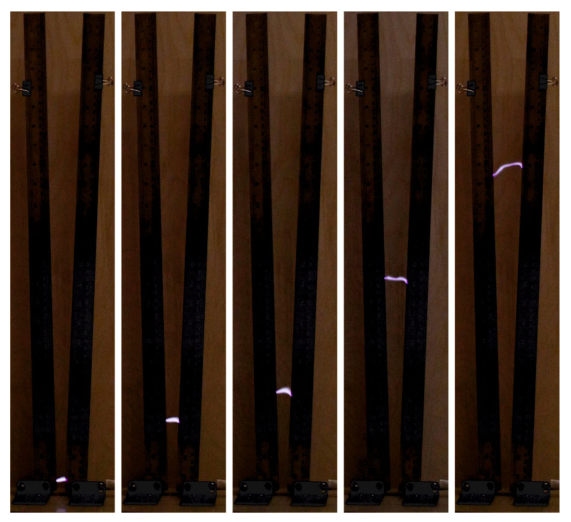
\includegraphics[width=0.3\textwidth]{figures/1.png}
    \caption{Experiment for Article II.}
\end{figure}

It was founded, that it moves with a constant velocity on most of the path. Also, the the dependence of the arc rise speed on the angle between the electrodes was investigated.


\section{Staged experiment (III articls)}


A slightly more meaningful experiment was set up in the next article, it has yet to be analyzed.

\begin{figure}[h]
    \centering
    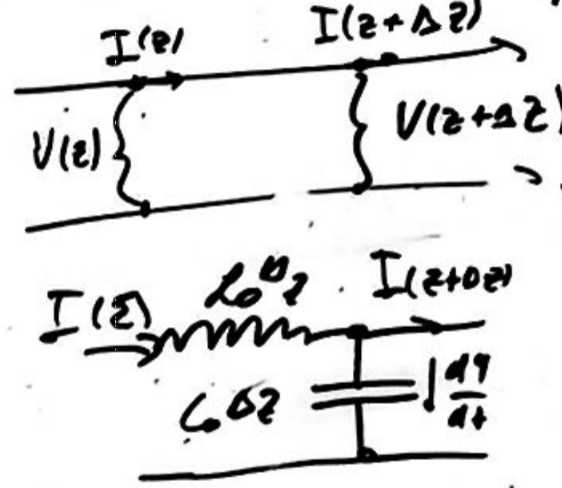
\includegraphics[width=0.4\textwidth]{figures/2.png}
    %\caption{}
    %\label{fig:}
\end{figure}





% % document's head
% \phantom{42}

\begin{center}
    \LARGE \textsc{Заметки курса <<Электричество и магнетизм>>}
\end{center}

\hrule

\phantom{42}

\begin{flushright}
    \begin{tabular}{rr}
    % written by:
        \textbf{Автор}: 
        & Хоружий Кирилл \\
        &\\
    % date:
        \textbf{От}: &
        \textit{\today}\\
    \end{tabular}
\end{flushright}

\thispagestyle{empty}
\tableofcontents
% \newpage


% \input
% \input







\end{document} Ну, что? Погнали техать?\begin{to_def} 
    \textit{Обобщенная сила} $Q_k$ -- величина коэффициента $\partial q^k$ при вариации $\delta A$, то есть $\delta A = Q_k \delta q^k$.
\end{to_def}

\begin{to_thr}[Уравнения Лагранжа второго рода]
     Каждая механическая система характеризуется определенной функцией $L(q, \dot{q}, t)$. Для голономных системы с конфигурационном многообразием степени $n$, верно что
     \begin{equation*}
         \frac{d}{dt} \frac{\partial L}{\partial \dot{q}_k} - \frac{\partial L}{\partial q_k} = 0, \hspace{0.5cm} k = 1, \ldots, n.
     \end{equation*}
     Где для потенциальных систем $L = T - \Pi$. В более общем случае можно записать, что
     \begin{equation*}
         \left(\frac{d }{d t} \frac{\partial T}{\partial \dot{q}^k} - \frac{\partial T}{\partial q^k} - Q^k\right)\delta q^k = 0, \hspace{0.5cm} 
         Q^k = - \frac{\partial \Pi}{\partial q^k}.
     \end{equation*}
\end{to_thr}

\begin{proof}[$\triangle$]
Запишем второй закон Ньютона:
$
    \left(
        m_i \vc{\mathrm{w}}_i = \vc{F}_i + \vc{R}_i
    \right)\big|_{\cdot \d \vc{r}_i}
$
, где $\vc{R}_i$ -- реакции связи. Хотим записать уравнение в общековариантном виде.
То есть мы <<замораживаем>> время, так чтобы $\vc{R} \cdot \delta \vc{r} = 0$. На таких перемещениях работа реакция связи равна 0.
\begin{align*}
    \bigg[
        \sum m_i \left(\vc{\mathrm{w}}_i \cdot \frac{\partial \vc{r}_i}{\partial q^k} \right)
        -
        \left(\vc{F}_i \cdot \frac{\partial \vc{r}_i}{\partial q^k} \right)
        -
        \underbrace{
        \left(
            \vc{R}_i \cdot \frac{\partial \vc{r}_i}{\partial q^k} 
        \right)}_{\cdot \delta q^k \to 0}
    \bigg] \cdot \delta q^k &= 0;
    \\
    \left[
        \frac{d}{dt} \frac{\partial }{\partial \dot{q}^k} \sum  \frac{m_i v_i^2}{2} 
        -
        \frac{\partial }{\partial q^k} \sum \frac{m_i v_i^2}{2} -
        \sum \vc{F}_i \frac{\partial \vc{r}_i}{\partial q^k} 
    \right] \delta q^k &= 0
    , \hspace{0.5cm} \Rightarrow \hspace{0.5cm} 
    \sum_k
    \left[
        \frac{d}{dt} \frac{\partial T}{\partial \dot{q}^k} 
        - \frac{\partial T}{\partial q^k} - Q^k
    \right] \delta q^k = 0.
\end{align*}
Проблема остается в неголономных системах, где $\delta q^k$ не являются независимыми, получается, что уравнения Лагранжа справедливы для голономных систем.

Вспоминая, что
\begin{equation*}
    \delta  A = \sum_i \vc{F}_i \cdot \delta \vc{r}_i =
    \sum_i \left(\vc{F}_i \cdot \frac{\partial \vc{r}_i}{\partial q^k}\right) \delta q^k =
    \sum_k 
    \frac{\delta A_k}{\delta q^k} \delta q^k = Q_k \delta q^k.
\end{equation*}
Тогда пусть $\Pi (q, t) \colon Q^k = - \partial \Pi / \partial q^k$.  Тогда
\begin{equation*}
    \frac{d}{dt} \frac{\partial (T-\Pi)}{\partial \dot{q}^k} - \frac{\partial (T - \Pi)}{\partial q^k}  = 0,
    \hspace{0.5cm} \Rightarrow \hspace{0.5cm} 
    \frac{d}{dt} \frac{\partial L}{\partial \dot{q}^k} - \frac{\partial L}{\partial q^k} = 0, \hspace{0.5cm} k = 1, \ldots, n.
\end{equation*}
То есть получили систему уравнений на $2n$ переменных.
\end{proof}



Подставим разложение кинетической энергии в уравнения Лагранжа, оставив только слагаемые с обобщёнными ускорениями $f_j (q, \dot{q}, t) = a_{jk} \ddot{q}^j$. 
\begin{equation*}
    T = \frac{1}{2} \sum_\nu m_\nu \dot{\vc{r}}_\nu^2 = \frac{1}{2} \sum_\nu
    \left(
        \frac{\partial \vc{r}_\nu}{\partial q^j} \dot{q}^j + \frac{\partial \vc{r}_\nu}{\partial t} 
    \right)^2 = 
    \frac{1}{2} 
    \bigg[
    \underbrace{
        a_{jk} \dot{q}^j \dot{q}^k
    }_{
        2T_2
    } +
    \underbrace{
        a_j \dot{q}^j
    }_{
        2T_1
    } +
    \underbrace{
        a_0
    }_{
        2T_0
    }
    \bigg],
\end{equation*}
где коэффициенты, соответственно, равны 
\begin{equation*}
    a_{jk}(q, t) = \sum_\nu m_\nu \frac{\partial \vc{r}_\nu}{\partial q^j} \cdot \frac{\partial \vc{r}_\nu}{\partial q^k},
    \hspace{0.5cm} 
    a_j(q, t) = \sum_\nu m_\nu \frac{\partial \vc{r}_\nu}{\partial q^j} \cdot \frac{\partial \vc{r}_\nu}{\partial t},
    \hspace{0.5cm} 
    a_0 = \sum_\nu m_\nu 
    \left(
    \frac{\partial \vc{r}_\nu}{\partial t} 
            \right)^2.
\end{equation*}
Для склерономных систем $\partial \vc{r}_\nu / \partial t = 0$, соотвественно $T = a_{jk} \dot{q}^j \dot{q}^k$, при чём $a_{jk} \equiv a_{jk} (q)$.

Теперь подставим значение $T$ в уравнения Лагранжа, и получим, что
$
    a_{ik} \ddot{q}^k = f_i,
$
где $f_1 = f_1(q, \dot{q}, t)$. Уравнений в системе $n$, причём $a_{jk}$ является положительно определенной формой\footnote{
    \red{Требует отдельного доказательства.}
}, соответственно невырожденной. 

\begin{to_thr} 
    Уравнения Лагранжа второго рода разрешимы относительно обобщенных ускорений 
\end{to_thr}
Пусть есть также непотенциальные силы, часть обобщенных сил, соответстующих непотенциальным силам, обозначим $Q_i^*$, тогда
\begin{equation*}
    Q_1 = - \frac{\partial \Pi}{\partial q^i} + Q_i^*,
    \hspace{0.5cm} \Rightarrow \hspace{0.5cm} 
    \frac{d }{d t} \frac{\partial T}{\partial \dot{q}^i} - 
    \frac{\partial T}{\partial q^i} 
    =
    - \frac{\partial \Pi}{\partial q^i} + Q_i^*.
\end{equation*}
Найдём производную по времени от кинетической энергии
\begin{equation*}
    \frac{d T}{d t} = 
    \frac{\partial T}{\partial \dot{q}^i} \ddot{q}^i + \frac{\partial T}{\partial q^i} \dot{q}_i + \frac{\partial T}{\partial t}  =
    \frac{d }{d t} \left(
        \frac{\partial T}{\partial \dot{q}^i} \dot{q}^i
    \right) - \left(
        \frac{d }{d t} \frac{\partial T}{\partial \dot{q}^i} - \frac{\partial T}{\partial q^i} 
    \right) \dot{q}^i + \frac{\partial T}{\partial t}.
\end{equation*}
По \textit{теореме Эйлера об однороных функциях} для $f(x_1, \ldots, x_n)$ $k$-й степени верно что
\begin{equation*}
    \frac{\partial f}{\partial x^i} x^i = kf,
    \hspace{0.5cm} \Rightarrow \hspace{0.5cm} 
    \frac{\partial T}{\partial \dot{q}^i} \dot{q}^i = 2 T_2 + T_1.
\end{equation*}
В таком случае последнее равеноство перепишется, как
\begin{align*}
    \frac{d T}{d t} 
    &=
    \frac{d }{d t} (2 T_2 + T_1) + \frac{\partial \Pi}{\partial q^i} \dot{q}^i - Q_i^* \dot{q}^i + \frac{\partial T}{\partial t} 
    = \\ &= 
    \frac{d }{d t} (2 T_2 + 2 T_1 + 2 T_0) - \frac{d }{d t} (T_1 + 2 T_0) + \frac{d \Pi}{d t} - \frac{\partial \Pi}{\partial t} - Q_i^* \dot{q}^i + \frac{\partial T}{\partial t}.
\end{align*}
Таким образом мы доказали следующую теорему.

\begin{to_thr}
     Полная мехническая энергия голономной системы $E = T+ \Pi$ изменяется следующим образом:
     \begin{equation*}
         \frac{d E}{d t} = N^* + \frac{d }{d t} (T_1 + 2 T_0) + \frac{\partial \Pi}{\partial t} - \frac{\partial T}{\partial t}.
     \end{equation*}
     Где $N^* = Q^*_i \dot{q}^i$ -- мощность непотенциальных сил.
\end{to_thr}


\begin{to_def} 
    Голономная склерономная система с  $\Pi \equiv \Pi(q)$ называется \textit{консервативной}, при чём $d E / d t = 0$.
\end{to_def}

\subsubsection*{Гироскопические силы}


\begin{to_def} 
    Непотенициальные силы называют \textit{гироскопическими}, если их мощность равна $0$. 
\end{to_def}


Пусть $Q^*_i = \gamma_{ik} \dot{q}^k$. Если $\gamma_{ik} = -\gamma_{ki}$, то силы $Q^*_i$ гиросокопические, соответсвенно кососимметричность $\gamma_{ik}$ необходима и достаточна.

Более того, имеет место равеноство

\vspace{-25pt}
\begin{equation*}
    \sum_\nu \vc{F}_\nu \cdot \vc{v}_\nu = \sum_\nu \vc{F}_\nu \cdot
    \left(
        \frac{\partial \vc{r}_\nu}{\partial q^i} \dot{q}^i + \frac{\partial \vc{r}_\nu}{\partial t} 
    \right) 
    =
     \bigg(
     \overbrace{
     \sum_\nu \vc{F}_\nu \cdot \frac{\partial \vc{r}_\nu}{\partial q^i}
     }^{
     Q_i
     }
      \bigg)
     \dot{q}^i + \sum_\nu \vc{F}_\nu \cdot \frac{\partial \vc{r}_\nu}{\partial t},
     \hspace{0.25cm} \overset{\partial \vv{r}_\nu / \partial t = 0}{=}  \hspace{0.25cm} 
     \sum_\nu \vc{F}_\nu \cdot \vc{v}_\nu = Q_i \dot{q}^i.
\end{equation*}
Поэтому для склерономных систем $N^* = 0$ выражается в $\sum_\nu \vc{F}_\nu^* \cdot \vc{v}_\nu = 0$.

\subsubsection*{Диссипативные силы}

\begin{to_def} 
    Непотенциальные силы называются диссипативными, если их $N^* \leq 0$, но $N^* \not \equiv 0$. При $\Pi = \Pi(q)$ и диссипативности сил $d E / dt \leq 0$, тогда система называется диссипативной. В случае определенно-отрицательной $N^* (\dot{q})$ дисспация называется \textit{полной}, а в случае знакопостоянной отрицательной $N^*$ \textit{частичной}.
\end{to_def}

\begin{to_def} 
    \textit{Диссипативной функцией Рэлея} называется  положительная квадратичная форма $R$ такая, что
    \begin{equation*}
        R = \frac{1}{2} b_{ik} \dot{q}^i \dot{q}^k,
        \hspace{1cm}
        Q^*_i = - \frac{\partial R}{\partial \dot{q}^i}  = - b_{ik} \dot{q}^k.
    \end{equation*}
    Тогда для склерономной системы можность $N^*$ непотенциальных сил равна
    \begin{equation*}
        \sum_\nu \vc{F}_\nu^* \cdot \vc{v}_\nu = Q_i^* \dot{q}^i = - 2 R \leq 0.
    \end{equation*}
\end{to_def}




Путь существует функция $V (q, \dot{q}, t)$ такая, что обобщенные силы $Q_i$ определяются по формулам
\begin{equation*}
    Q_i = \frac{d }{d t} \frac{\partial V}{\partial \dot{q}^i} - \frac{\partial V}{\partial q^i}.
\end{equation*}
Тогда функция $V$ называется обобщенным потенциалом. Действительно, при $L = T - V$ уравнения движения запишутся в той же форме. Дифференцируя по времени выясним, что
\begin{equation*}
    Q_i = \frac{\partial^2 V}{\partial \dot{q}^i \partial \dot{q}^k} \ddot{q}^k + f_i,
\end{equation*}
где $f_i \equiv f_i ( q,\dot{q}, t)$. Но так как зависимость $Q_i(\ddot{q})$ это странно, то
\begin{equation*}
    V =  A_i(q, t) \dot{q}^i + V_0(q, t).
\end{equation*}
Тогда обобщенные силы
\begin{equation*}
    Q_i = \frac{d A_i}{d t} - \frac{\partial }{\partial q^i} \left(
        A_k \dot{q}^k  + V_0
    \right) = - \frac{\partial V_0}{\partial q^i} + \frac{\partial A_i}{\partial t} +
    \left(
        \frac{\partial A_i}{\partial q^k} - \frac{\partial A_k}{\partial q^i} 
    \right) \dot{q}^k.
\end{equation*}
Если $\partial A_i / \partial t = 0$, то $Q_i$ складываются из потенциальных $\partial V_0 / \partial q_i$ и гироскопических $Q_i^* = \gamma_{ik} \dot{q}^k$, где $\gamma_{ik} = \partial_k A_i - \partial_i A_k$. Если система склерономна и $V_0 \neq V_0(t)$, то $T+V_0$ остается постоянной.

В случае существования обобщенного потенциала $L$ всё так же многочлен второй степени относительно $q, \ \dot{q}$, при чём $L_2 = T_2$, так что уравнения остаются разрешимы относительно обобщенных ускорений.









\begin{to_def} 
    \textit{Действием по Гамильтону} называют функционал вида
    \begin{equation*}
         S = \int_{t_0}^{t_1} L(\gamma(t), \dot{\gamma}(t), t) \d t.
    \end{equation*} 
    Переходя к однопараметрическому семейству кривых $\gamma(\alpha, t)$ получим \textit{вариацию действия}
    \begin{equation*}
        S = \int_{t_0}^{t_1} L(\gamma(\alpha, t), \dot{\gamma}(\alpha, t), t) \d t, 
        \hspace{0.5cm} 
        \delta S = \frac{d S}{d \alpha} \delta \alpha.
    \end{equation*}
\end{to_def}


\begin{to_thr}[принцип Гамильтона]
    Кривая $\gamma(\alpha, t)$ является экстремалью действия тогда и только тогда, когда является решением уравнений Лагранжа
     \begin{equation*}
         \delta S = 0
         \hspace{0.5cm} \Leftrightarrow \hspace{0.5cm} 
         \gamma(\alpha, t) \in \textnormal{Sol}\,
         \left(
     \frac{d}{dt} \frac{\partial L}{\partial \dot{q}^k} - \frac{\partial L}{\partial q^k} = 0
         \right)
         .
     \end{equation*}
\end{to_thr}


\begin{proof}[$\triangle$]
    Давайте просто проварьируем Лагранжиан, тогда
    \begin{align*}
        \delta S 
        &=
         \int_{t_0}^{t_1} 
        \left(
            \frac{\partial L}{\partial q^i} \frac{\partial q^i}{\partial \alpha} +
            \frac{\partial L}{\partial \dot{q}^i} \frac{\partial \dot{q}^i}{\partial \alpha}  
        \right) \delta \alpha \d t 
        =
        \int_{t_0}^{t_1} \left(
            \frac{\partial L}{\partial q^i} \delta q^i + \frac{\partial L}{\partial \dot{q}^i} \delta \dot{q}^i
        \right) \d t
        =
        \frac{\partial L}{\partial \dot{q}} \partial q \bigg|_{t_1}^{t_2}
        + \int_{t_1}^{t_2}
        \left(
            \frac{\partial L}{\partial q^i} - \frac{d }{d t} \frac{\partial L}{\partial \dot{q}^i} 
        \right) \,\delta q^i \d t
        = 0.
    \end{align*}
    таким образом уравнения Лагранжа выполнены. 
\end{proof}

% в первых билет засунуть конфигурационное многообразие
\definecolor{grey}{HTML}{666666}
\definecolor{linkcolor}{HTML}{0000CC}
\definecolor{urlcolor}{HTML}{006600}
\hypersetup{
    pdfstartview=FitH,  
    linkcolor=linkcolor,
    urlcolor=urlcolor, 
    colorlinks=true,
    citecolor=blue}% add (renew) commands

\renewcommand{\Im}{\mathop{\mathrm{Im}}\nolimits}
\renewcommand{\Re}{\mathop{\mathrm{Re}}\nolimits}
\renewcommand{\d}{\, d}
\renewcommand{\leq}{\leqslant}
\renewcommand{\geq}{\geqslant}
\renewcommand{\L}{\mathcal{L}}


\newcommand{\vc}[1]{\mbox{\boldmath $#1$}}
\newcommand{\T}{^{\text{T}}}

\newcommand{\incfig}[1]{%
    \def\svgwidth{\columnwidth}
    \import{./figures/}{#1.pdf_tex}
}

\newcommand{\diag}{\mathop{\mathrm{diag}}\nolimits}
\newcommand{\id}{\mathop{\mathrm{id}}\nolimits}
\newcommand{\grad}{\mathop{\mathrm{grad}}\nolimits}
\renewcommand{\div}{\mathop{\mathrm{div}}\nolimits}
\newcommand{\rot}{\mathop{\mathrm{rot}}\nolimits}
\newcommand{\Ker}{\mathop{\mathrm{Ker}}\nolimits}
\newcommand{\Spec}{\mathop{\mathrm{Spec}}\nolimits}
\newcommand{\sign}{\mathop{\mathrm{sign}}\nolimits}
\newcommand{\tr}{\mathop{\mathrm{tr}}\nolimits}
\newcommand{\rg}{\mathop{\mathrm{rg}}\nolimits}

\newcommand{\const}{\text{const}}
\newcommand{\red}[1]{\textcolor{red}{#1}}
\newcommand{\xmark}{\ding{55}}

\newcommand{\sbsnum}[2]{
    \setcounter{subsection}{\the\numexpr #1 - 1 \relax}
    \subsection{#2}
}
\newcommand{\secnum}[2]{
    \section*{#2}
    \setcounter{section}{#1}
    \addcontentsline{toc}{section}{#2}
}


\newcommand{\set}[2]{{#1}^{1}, \ldots, {#1}^{#2}}
\newtheorem{to_thr}{Thr}[subsection]
\newtheorem{to_suj}[to_thr]{Suj}
\newtheorem{to_lem}[to_thr]{Lem}
\newtheorem{to_com}[to_thr]{Com}
\newtheorem{to_con}[to_thr]{Con}
\theoremstyle{definition}
\newtheorem{to_def}[to_thr]{Def}
\newtheorem{to_tas}[to_thr]{Task}
\newtheorem{to_exm}[to_thr]{Exm}


\newenvironment{itemize*}
{
    \begin{itemize}
        \setlength{\itemsep}{1pt}
        \setlength{\parskip}{1pt}}
    {\end{itemize}
}

\newenvironment{enumerate*}
{
    \begin{enumerate}
        \setlength{\itemsep}{1pt}
        \setlength{\parskip}{1pt}}
    {\end{enumerate}
}

\newenvironment{description*}
{
    \begin{description}
        \setlength{\itemsep}{1pt}
        \setlength{\parskip}{1pt}}
    {\end{description}
}% add page header

\pagestyle{fancy}
\fancyhf{}
\fancyhead[RE,LO]{\textsc{Ф\raisebox{-1.5pt}{и}з\TeX}}
\fancyhead[LE,RO]{Ж\raisebox{-1.5pt}{и}К}
% \fancyhead[CO,CE]{\leftmark}
\fancyfoot[LE,RO]{\textcolor{grey}{\texttt{\thepage}}}

% document's head
% \phantom{42}

\begin{center}
    \LARGE \textsc{Билеты к экзамену по <<Аналитической Механике>>, ФОПФ}
\end{center}

\hrule

\phantom{42}

\begin{flushright}
    \begin{tabular}{rr}
    % written by:
        \textbf{Авторы}: 
        & Хоружий Кирилл \\
        & Примак Евгений \\
        &\\
    % date:
        \textbf{От}: &
        \textit{\today}\\
    \end{tabular}
\end{flushright}

\thispagestyle{empty}
\tableofcontents
\newpage% input files

% document's head
% \phantom{42}

\begin{center}
    \LARGE \textsc{Заметки курса <<Электричество и магнетизм>>}
\end{center}

\hrule

\phantom{42}

\begin{flushright}
    \begin{tabular}{rr}
    % written by:
        \textbf{Автор}: 
        & Хоружий Кирилл \\
        &\\
    % date:
        \textbf{От}: &
        \textit{\today}\\
    \end{tabular}
\end{flushright}

\thispagestyle{empty}
\tableofcontents
% \newpage


\sbsnum{31}{Уравнение Лагранжа второго рода}
\begin{to_lem}[Разбиение единицы в окрестности компакта на многообразии]
     Пусть $M$ -- гладкое многообразие, а $K \subseteq M$ -- его компактное подмножество. Для любого покрытия $\{U_\alpha\}_\alpha$ компакта $K$ открытыми множествами найдётся набор неотрицательных гладких функций $\{\rho_\alpha\}_\alpha$ с компактными носителями $\mathrm{supp}\, \rho_\alpha$ таких, что
\begin{equation*}
    \forall \alpha \ \textnormal{supp}\, \rho_\alpha \subset U_\alpha,
\end{equation*}
    только конечное число из них отлично от нуля и
    $\sum_\alpha \rho_\alpha (x) \equiv 1$
    в некоторой окрестности $K$.
\end{to_lem}

\begin{to_def} 
    Интеграл дифференциальной формы $\nu \in \Omega_{\text{c}}^n (M)$ с компактным носителем по ориентированному $n$-мерному многообразию $M$ определяется с помощью разбиения единицы в окрестности носителя $\nu$ 
    \begin{equation*}
         \rho_1 + \ldots + \rho_m = 1,
     \end{equation*} 
     подчиненного некоторому набору положительно ориентрированных карт как
     \begin{equation*}
         \int_M \nu = \sum_i \int_M \rho_i \nu_i,
     \end{equation*}
     где интегралы справа рассматриваются в координатных картах, содержащих носители соответствующих $\rho_i$.
\end{to_def}

\begin{to_lem} 
    Определение интеграла не зависит от выбора системы положительных карт в данной ориентации и подчиненного им разбиения единциы. 
\end{to_lem}





\sbsnum{32}{Разрешимость уравнений Лагранжа}
Подставим разложение кинетической энергии в уравнения Лагранжа, оставив только слагаемые с обобщёнными ускорениями $f_j (q, \dot{q}, t) = a_{jk} \ddot{q}^j$. 
\begin{equation*}
    T = \frac{1}{2} \sum_\nu m_\nu \dot{\vc{r}}_\nu^2 = \frac{1}{2} \sum_\nu
    \left(
        \frac{\partial \vc{r}_\nu}{\partial q^j} \dot{q}^j + \frac{\partial \vc{r}_\nu}{\partial t} 
    \right)^2 = 
    \frac{1}{2} 
    \bigg[
    \underbrace{
        a_{jk} \dot{q}^j \dot{q}^k
    }_{
        2T_2
    } +
    \underbrace{
        a_j \dot{q}^j
    }_{
        2T_1
    } +
    \underbrace{
        a_0
    }_{
        2T_0
    }
    \bigg],
\end{equation*}
где коэффициенты, соответственно, равны 
\begin{equation*}
    a_{jk}(q, t) = \sum_\nu m_\nu \frac{\partial \vc{r}_\nu}{\partial q^j} \cdot \frac{\partial \vc{r}_\nu}{\partial q^k},
    \hspace{0.5cm} 
    a_j(q, t) = \sum_\nu m_\nu \frac{\partial \vc{r}_\nu}{\partial q^j} \cdot \frac{\partial \vc{r}_\nu}{\partial t},
    \hspace{0.5cm} 
    a_0 = \sum_\nu m_\nu 
    \left(
    \frac{\partial \vc{r}_\nu}{\partial t} 
            \right)^2.
\end{equation*}
Для склерономных систем $\partial \vc{r}_\nu / \partial t = 0$, соотвественно $T = a_{jk} \dot{q}^j \dot{q}^k$, при чём $a_{jk} \equiv a_{jk} (q)$.

Теперь подставим значение $T$ в уравнения Лагранжа, и получим, что
$
    a_{ik} \ddot{q}^k = f_i,
$
где $f_1 = f_1(q, \dot{q}, t)$. Уравнений в системе $n$, причём $a_{jk}$ является положительно определенной формой\footnote{
    \red{Требует отдельного доказательства.}
}, соответственно невырожденной. 

\begin{to_thr} 
    Уравнения Лагранжа второго рода разрешимы относительно обобщенных ускорений 
\end{to_thr}


\sbsnum{33}{Изменение полной мехнической энергии голономной системы}
Пусть есть также непотенциальные силы, часть обобщенных сил, соответстующих непотенциальным силам, обозначим $Q_i^*$, тогда
\begin{equation*}
    Q_1 = - \frac{\partial \Pi}{\partial q^i} + Q_i^*,
    \hspace{0.5cm} \Rightarrow \hspace{0.5cm} 
    \frac{d }{d t} \frac{\partial T}{\partial \dot{q}^i} - 
    \frac{\partial T}{\partial q^i} 
    =
    - \frac{\partial \Pi}{\partial q^i} + Q_i^*.
\end{equation*}
Найдём производную по времени от кинетической энергии
\begin{equation*}
    \frac{d T}{d t} = 
    \frac{\partial T}{\partial \dot{q}^i} \ddot{q}^i + \frac{\partial T}{\partial q^i} \dot{q}_i + \frac{\partial T}{\partial t}  =
    \frac{d }{d t} \left(
        \frac{\partial T}{\partial \dot{q}^i} \dot{q}^i
    \right) - \left(
        \frac{d }{d t} \frac{\partial T}{\partial \dot{q}^i} - \frac{\partial T}{\partial q^i} 
    \right) \dot{q}^i + \frac{\partial T}{\partial t}.
\end{equation*}
По \textit{теореме Эйлера об однороных функциях} для $f(x_1, \ldots, x_n)$ $k$-й степени верно что
\begin{equation*}
    \frac{\partial f}{\partial x^i} x^i = kf,
    \hspace{0.5cm} \Rightarrow \hspace{0.5cm} 
    \frac{\partial T}{\partial \dot{q}^i} \dot{q}^i = 2 T_2 + T_1.
\end{equation*}
В таком случае последнее равеноство перепишется, как
\begin{align*}
    \frac{d T}{d t} 
    &=
    \frac{d }{d t} (2 T_2 + T_1) + \frac{\partial \Pi}{\partial q^i} \dot{q}^i - Q_i^* \dot{q}^i + \frac{\partial T}{\partial t} 
    = \\ &= 
    \frac{d }{d t} (2 T_2 + 2 T_1 + 2 T_0) - \frac{d }{d t} (T_1 + 2 T_0) + \frac{d \Pi}{d t} - \frac{\partial \Pi}{\partial t} - Q_i^* \dot{q}^i + \frac{\partial T}{\partial t}.
\end{align*}
Таким образом мы доказали следующую теорему.

\begin{to_thr}
     Полная мехническая энергия голономной системы $E = T+ \Pi$ изменяется следующим образом:
     \begin{equation*}
         \frac{d E}{d t} = N^* + \frac{d }{d t} (T_1 + 2 T_0) + \frac{\partial \Pi}{\partial t} - \frac{\partial T}{\partial t}.
     \end{equation*}
     Где $N^* = Q_i^* \dot{q}^i$ -- мощность непотенциальных сил.
\end{to_thr}


\begin{to_def} 
    Голономная склерономная система с  $\Pi \equiv \Pi(q)$ называется \textit{консервативной}, при чём $d E / d t = 0$.
\end{to_def}

\subsubsection*{Гироскопические силы}


\begin{to_def} 
    Непотенициальные силы называют \textit{гироскопическими}, если их мощность равна $0$. 
\end{to_def}


Пусть $Q_i^* = \gamma_{ik} \dot{q}^k$. Если $\gamma_{ik} = -\gamma_{ki}$, то силы $Q_i^*$ гиросокопические, соответсвенно кососимметричность $\gamma_{ik}$ необходима и достаточна.

Более того, имеет место равеноство

\vspace{-25pt}
\begin{equation*}
    \sum_\nu \vc{F}_\nu \cdot \vc{v}_\nu = \sum_\nu \vc{F}_\nu \cdot
    \left(
        \frac{\partial \vc{r}_\nu}{\partial q^i} \dot{q}^i + \frac{\partial \vc{r}_\nu}{\partial t} 
    \right) 
    =
     \bigg(
     \overbrace{
     \sum_\nu \vc{F}_\nu \cdot \frac{\partial \vc{r}_\nu}{\partial q^i}
     }^{
     Q_i
     }
      \bigg)
     \dot{q}^i + \sum_\nu \vc{F}_\nu \cdot \frac{\partial \vc{r}_\nu}{\partial t},
     \hspace{0.25cm} \overset{\partial \vv{r}_\nu / \partial t = 0}{=}  \hspace{0.25cm} 
     \sum_\nu \vc{F}_\nu \cdot \vc{v}_\nu = Q_i \dot{q}^i.
\end{equation*}
Поэтому для склерономных систем $N^* = 0$ выражается в $\sum_\nu \vc{F}_\nu^* \cdot \vc{v}_\nu = 0$.

\subsubsection*{Диссипативные силы}

\begin{to_def} 
    Непотенциальные силы называются диссипативными, если их $N^* \leq 0$, но $N^* \not \equiv 0$. При $\Pi = \Pi(q)$ и диссипативности сил $d E / dt \leq 0$, тогда система называется диссипативной. В случае определенно-отрицательной $N^* (\dot{q})$ дисспация называется \textit{полной}, а в случае знакопостоянной отрицательной $N^*$ \textit{частичной}.
\end{to_def}

\begin{to_def} 
    \textit{Диссипативной функцией Рэлея} называется  положительная квадратичная форма $R$ такая, что
    \begin{equation*}
        R = \frac{1}{2} b_{ik} \dot{q}^i \dot{q}^k,
        \hspace{1cm}
        Q_i^* = - \frac{\partial R}{\partial \dot{q}^i}  = - b_{ik} \dot{q}^k.
    \end{equation*}
    Тогда для склерономной системы можность $N^*$ непотенциальных сил равна
    \begin{equation*}
        \sum_\nu \vc{F}_\nu^* \cdot \vc{v}_\nu = Q_i^* \dot{q}^i = - 2 R \leq 0.
    \end{equation*}
\end{to_def}






\sbsnum{34}{Обобщенный потенциал и первые интегралы лагранжевых систем}
Физический потенциал силового поля в математический терминах означает поиск $f \in C^\infty (M) \colon \d f = \alpha$ для заданной силы $\alpha \in \Omega^1(M)$

\begin{to_def} 
	Пусть $\vc{A}$ -- векторное поле в области $D \subset \mathbb{R}^n$. Функция $U \colon D \mapsto \mathbb{R}$ называется \textit{потенциалом поля} $\vc{A}$ в области $D$, если в этой области $\vc{A} = \grad U$. Поле, обладающее потенциалом, называется \textit{потенциальным полем}. 
\end{to_def}

\begin{to_thr}
	Необходимым и достаточным условием наличия потенциала у непрерывной $\alpha \in \Omega^1(M)$, для гладкого $M$, является независимость $\int_\gamma \alpha$ от выбора  кусочно-гладкой кривой $\gamma$ между двумя точками.

	Эквивалентно можно потребовать равенства нулю интегралов по всем замкнутым кусочно-гладким кривым.
	\label{thr_7.1}
\end{to_thr}

\begin{to_lem}[Необходимое условие потенциальности]
	 Необходимым условием существования потенциала у $\alpha \in \Omega^1(M)$ является $\d \alpha = 0$ (т.к. $\d (\d u) = 0$).
\end{to_lem}

\begin{to_lem} 
	В случае $\mathbb{R}^3$ по определению $d \omega^1_{\vv{A}} = \omega^2_{\rot \vv{A}}$, поэтому необходимое условие потенциальности поля $\vc{A}$ переписывается в виде $\rot \vc{A} = 0$.
\end{to_lem}

Однако этого не достаточно, так например в открытой $U = \mathbb{R}^2 \backslash \{ 0 \}$:
\begin{equation*}
	\alpha = \frac{x \d y - y \d x}{x^2 + y^2}
	\hspace*{0.5 cm} \leadsto \hspace*{0.5 cm}
	\d \alpha = 0,
	\hspace*{0.5 cm} \text{ но } \hspace*{0.5 cm}
	\oint_{S^1} \alpha = 2 \pi.
\end{equation*}


\begin{to_def} 
	Поле $\vc{A}$ называется \textit{векторным потенциалом} поля $\vc{B}$ в области $D \subset \mathbb{R}^3$, если в этой области выполняется соотношение $\vc{B} = \rot \vc{A}$. 
\end{to_def}

Это можно переписать в виде $\omega^2_{\vv{B}} = d \omega^1_{\vv{A}}$, тогда $\omega^3_{\div \vv{B}} = d \omega_{\vv{B}}^2 = d^2 \omega^1_{\vv{A}} = 0$, то есть необходимое условие $\div \vc{B} = 0$, принято такое поле называть \textit{соленоидальным}. 









% \sbsnum{36}{Принцип наименьшего действия}
% В силу теоремы Пуанкаре (\ref{thr_poin}) любая замкнутая форма на многообразии локально точна, однако склеивать их в точную на всём пространство нам будут мешать дырки, как это случалось в задаче из нашего задания.
Связь между устройством многообразия и взаимоотношением  замкнутых и точных форм на нём описывается группами (ко)гомологий де Рама.

Замкнутые и точные формы на $M$ образуют линейные пространства $Z^k(M)$ и $B^k(M)$ соответственно.

\begin{to_def}[Когомологии де Рама] или группа $k$-мерных когомологий многообразия $M$:
	\begin{equation*}
		H^k(M) = Z^k(M)/B^k(M).
	\end{equation*}
\end{to_def}

\begin{to_def}
	Если формы $\alpha_1, \alpha_2$ отличаются на точную форму, то говорят, что они гомологичны.
	\label{def_7.16}
\end{to_def}
Таким образом если замкнутые $\alpha_1, \alpha_2$ гомологичны, то они лежат в одном классе когомологии.

По скольку $Z^k (M)$ есть $\Ker d \colon \Omega^k(M) \rightarrow \Omega^{k+1}(M)$, а $B^k (M)$ есть $\Im d \colon \Omega^{k-1}(M) \rightarrow \Omega^{k}(M)$, то часто переписывают:

\begin{to_def}
	Когомологии де Рама гладкого $M$ --- это факторпространства
	\begin{equation*}
		H_{DR}^k (M) = \frac{\Ker d \colon \Omega^k(M) \rightarrow \Omega^{k+1}(M)}{\Im d \colon \Omega^{k-1}(M) \rightarrow \Omega^{k}(M)}.
	\end{equation*}
	\label{def_7.17}
\end{to_def}

\begin{to_lem}[Лемма Пуанкаре]
	\begin{equation*}
		H^p(\mathbb{R}^k) = 0 \text{ при } k>0,
		\hspace*{1 cm}  \hspace*{1 cm}
		H^k(\mathbb{R}^k) \sim \mathbb{R} \text{ при } k=0.
	\end{equation*}
	\label{lem_7.19}
\end{to_lem}\newcommand{\dmat}[4]{
  \ifthenelse{
    \equal{#1}{3}
  }{
\begin{pmatrix}
    #2 & 0 & 0 \\
    0 & #3 & 0 \\
    0 & 0 & #4 \\
\end{pmatrix}
  }{
  \ifthenelse{
      \equal{#1}{2}
    }{
  \begin{pmatrix}
      #2 & 0 \\
      0 & #3 \\
  \end{pmatrix}
    }{
      \text{\textcolor{red}{error}}
    }
  }
}

\newcommand{\skmat}[4]{
  \ifthenelse{
    \equal{#1}{3}
  }{
\begin{pmatrix}
    0 & -#4 & #3 \\
    #4 & 0 & -#2 \\
    -#3 & #2 & 0 \\
\end{pmatrix}
  }{
  \ifthenelse{
      \equal{#1}{2}
    }{
  \begin{pmatrix}
      0 & #2 \\
      -#2 & 0 \\
  \end{pmatrix}
    }{
      \text{\textcolor{red}{error}}
    }
  }
}
\usepackage[T2A]{fontenc}                   %!? закрепляет внутреннюю кодировку LaTeX
\usepackage[utf8]{inputenc}                 %!  закрепляет кодировку utf8
\usepackage[english,russian]{babel}         %!  подключает русский и английский
\usepackage[margin=1.7cm]{geometry}         %!  фиксирует оступ на 2cm

\usepackage[unicode, pdftex]{hyperref}      %!  оглавление для панели навигации по PDF-документу + гиперссылки

\usepackage{amsthm}                         %!  newtheorem и их сквозная нумерация
\usepackage{hypcap}                         %?  адресация на картинку, а не на подпись к ней
\usepackage{caption}                        %-  позволяет корректировать caption 
\usepackage{fancyhdr}                       %   добавить верхний и нижний колонтитул
\usepackage{wrapfig}                        %!  обтекание таблиц и рисунков

\usepackage{amsmath}                        %!  |
\usepackage{amssymb,textcomp, esvect,esint} %!  |важно для формул 
\usepackage{amsfonts}                       %!  математические шрифты
\usepackage{mathrsfs}                       %  добавит красивые E, H, L
\usepackage{ulem}                           %!  перечеркивание текста
\usepackage{abraces}                        %?  фигурные скобки сверху или снизу текста
\usepackage{pifont}                         %!  нужен для крестика
\usepackage{cancel}                         %!  аутентичное перечеркивание текста
\usepackage{esvect}                         %  добавит вектора стрелочками

\usepackage{graphicx}                       %?  графическое изменение текста
\usepackage{indentfirst}                    %   добавить indent перед первым параграфом
\usepackage{xcolor}                         %   добавляет цвета
\usepackage{enumitem}                       %!  задание макета перечня.

\usepackage{booktabs}                       %!  добавляет книжные линии в таблицы
\usepackage{multirow}                       %   объединение ячеек в таблицах

\usepackage{tikz}                           %!  высокоуровневые рисунки (кружочек)

\usepackage{import}                         %   |
\usepackage{xifthen}                        %   |
\usepackage{pdfpages}                       %   | вставка рисунков pdf_tex
\usepackage{transparent}                    %   |

\setlength{\headheight}{12.52pt}            % избегать warning

\usepackage{chngcntr}
\renewcommand\thesubsection{\arabic{subsection}}
\counterwithout{equation}{section}

\renewcommand{\theequation}{\arabic{equation}}
% \usepackage[upint]{stix}% file's preambule
%%%%%%%%%%%%%%%%%%%



% connect packages

\usepackage[T2A]{fontenc}                   %!? закрепляет внутреннюю кодировку LaTeX
\usepackage[utf8]{inputenc}                 %!  закрепляет кодировку utf8
\usepackage[english,russian]{babel}         %!  подключает русский и английский
\usepackage[margin=1.7cm]{geometry}         %!  фиксирует оступ на 2cm

\usepackage[unicode, pdftex]{hyperref}      %!  оглавление для панели навигации по PDF-документу + гиперссылки

\usepackage{amsthm}                         %!  newtheorem и их сквозная нумерация
\usepackage{hypcap}                         %?  адресация на картинку, а не на подпись к ней
\usepackage{caption}                        %-  позволяет корректировать caption 
\usepackage{fancyhdr}                       %   добавить верхний и нижний колонтитул
\usepackage{wrapfig}                        %!  обтекание таблиц и рисунков

\usepackage{amsmath}                        %!  |
\usepackage{amssymb,textcomp, esvect,esint} %!  |важно для формул 
\usepackage{amsfonts}                       %!  математические шрифты
\usepackage{mathrsfs}                       %  добавит красивые E, H, L
\usepackage{ulem}                           %!  перечеркивание текста
\usepackage{abraces}                        %?  фигурные скобки сверху или снизу текста
\usepackage{pifont}                         %!  нужен для крестика
\usepackage{cancel}                         %!  аутентичное перечеркивание текста
\usepackage{esvect}                         %  добавит вектора стрелочками

\usepackage{graphicx}                       %?  графическое изменение текста
\usepackage{indentfirst}                    %   добавить indent перед первым параграфом
\usepackage{xcolor}                         %   добавляет цвета
\usepackage{enumitem}                       %!  задание макета перечня.

\usepackage{booktabs}                       %!  добавляет книжные линии в таблицы
\usepackage{multirow}                       %   объединение ячеек в таблицах

\usepackage{tikz}                           %!  высокоуровневые рисунки (кружочек)

\usepackage{import}                         %   |
\usepackage{xifthen}                        %   |
\usepackage{pdfpages}                       %   | вставка рисунков pdf_tex
\usepackage{transparent}                    %   |

\setlength{\headheight}{12.52pt}            % избегать warning

% create environment

\newtheorem{to_thr}{Thr}[subsection]
\newtheorem{to_suj}[to_thr]{Suj}
\newtheorem{to_lem}[to_thr]{Lem}
\newtheorem{to_com}[to_thr]{Com}
\newtheorem{to_con}[to_thr]{Con}
\theoremstyle{definition}
\newtheorem{to_def}[to_thr]{Def}
\newtheorem{to_tas}[to_thr]{Task}
\newtheorem{to_exm}[to_thr]{Exm}


\newenvironment{itemize*}
{
    \begin{itemize}
        \setlength{\itemsep}{1pt}
        \setlength{\parskip}{1pt}}
    {\end{itemize}
}

\newenvironment{enumerate*}
{
    \begin{enumerate}
        \setlength{\itemsep}{1pt}
        \setlength{\parskip}{1pt}}
    {\end{enumerate}
}

\newenvironment{description*}
{
    \begin{description}
        \setlength{\itemsep}{1pt}
        \setlength{\parskip}{1pt}}
    {\end{description}
}

% document palette

\definecolor{grey}{HTML}{666666}
\definecolor{linkcolor}{HTML}{0000CC}
\definecolor{urlcolor}{HTML}{006600}
\hypersetup{
    pdfstartview=FitH,  
    linkcolor=linkcolor,
    urlcolor=urlcolor, 
    colorlinks=true,
    citecolor=blue}

% add (renew) commands
% add (renew) commands

\renewcommand{\Im}{\mathop{\mathrm{Im}}\nolimits}
\renewcommand{\Re}{\mathop{\mathrm{Re}}\nolimits}
\renewcommand{\d}{\, d}
\renewcommand{\leq}{\leqslant}
\renewcommand{\geq}{\geqslant}

\newcommand{\vc}[1]{\mbox{\boldmath $#1$}}
\newcommand{\T}{^{\text{T}}}

\newcommand{\incfig}[1]{%
    \def\svgwidth{\columnwidth}
    \import{./figures/}{#1.pdf_tex}
}

\newcommand{\diag}{\mathop{\mathrm{diag}}\nolimits}
\newcommand{\grad}{\mathop{\mathrm{grad}}\nolimits}
\renewcommand{\div}{\mathop{\mathrm{div}}\nolimits}
\newcommand{\rot}{\mathop{\mathrm{rot}}\nolimits}
\newcommand{\Ker}{\mathop{\mathrm{Ker}}\nolimits}
\newcommand{\Spec}{\mathop{\mathrm{Spec}}\nolimits}
\newcommand{\sign}{\mathop{\mathrm{sign}}\nolimits}
\newcommand{\tr}{\mathop{\mathrm{tr}}\nolimits}
\newcommand{\rg}{\mathop{\mathrm{rg}}\nolimits}

\newcommand{\const}{\text{const}}
\newcommand{\red}[1]{\textcolor{red}{#1}}
\newcommand{\xmark}{\ding{55}}


\newcommand{\sbsnum}[2]{
    \setcounter{subsection}{\the\numexpr #1 - 1 \relax}
    \subsection{#2}
}


% add page header
% add page header

\pagestyle{fancy}
\fancyhf{}
\fancyhead[RE,LO]{\textsc{Ф\raisebox{-1.5pt}{и}з\TeX}}
\fancyhead[LE,RO]{НАЗВАНИЕ}
\fancyhead[CO,CE]{\leftmark}
\fancyfoot[LE,RO]{\textcolor{grey}{\texttt{\thepage}}}



% matrixes shortcuts 
\newcommand{\dmat}[4]{
  \ifthenelse{
    \equal{#1}{3}
  }{
\begin{pmatrix}
    #2 & 0 & 0 \\
    0 & #3 & 0 \\
    0 & 0 & #4 \\
\end{pmatrix}
  }{
  \ifthenelse{
      \equal{#1}{2}
    }{
  \begin{pmatrix}
      #2 & 0 \\
      0 & #3 \\
  \end{pmatrix}
    }{
      \text{\textcolor{red}{error}}
    }
  }
}

\newcommand{\skmat}[4]{
  \ifthenelse{
    \equal{#1}{3}
  }{
\begin{pmatrix}
    0 & -#4 & #3 \\
    #4 & 0 & -#2 \\
    -#3 & #2 & 0 \\
\end{pmatrix}
  }{
  \ifthenelse{
      \equal{#1}{2}
    }{
  \begin{pmatrix}
      0 & #2 \\
      -#2 & 0 \\
  \end{pmatrix}
    }{
      \text{\textcolor{red}{error}}
    }
  }
}

% additional symbols and commands


\DeclareRobustCommand{\tmpsim}{ %%%%%%%%%%%%%% ~ < %%%%%%%%%%%%%%%%%%%
  \mathbin{\text{
      \raisebox{-1pt}{
            \hspace{-4.5pt} \rotatebox{-26}{\scalebox{0.8}[0.7]{$\sim$}}
        }
  }}
}
\def\lesim{{
    \setbox0\hbox{$\ <\ $}
    \rlap{\hbox to \wd0{\hss$\tmpsim$\hss}}\box0
}}
%%%%%%%%%%%%%%%%%%%%%%%%%%%%%%%%%%%%%%%%%%%%%%%%%%%%%%%%%%%%%%%%%%%%%%


\def\letuscom{%%%%%%%%%%%%%%%%%%%%%% ПУСТЬ %%%%%%%%%%%%%%%%%%%%%%%%%%
\mathord{\setbox0=\hbox{$\exists$}%
     \hbox{\kern 0.125\wd0%
           \vbox to \ht0{%
              \hrule width 0.75\wd0%
              \vfill%
              \hrule width 0.75\wd0}%
           \vrule height \ht0%
           \kern 0.125\wd0}%
   }%
}
\newcommand{\letus}{\raisebox{-1.2pt}{$\letuscom$}}
%%%%%%%%%%%%%%%%%%%%%%%%%%%%%%%%%%%%%%%%%%%%%%%%%%%%%%%%%%%%%%%%%%%%%%


\usepackage{arydshln} %%%%%%%%%%%%%%% ЛИНИИ В МАТРИЧКЕ %%%%%%%%%%%%%%%
\makeatletter
  \renewcommand*\env@matrix[1][*\c@MaxMatrixCols c]{%
    \hskip -\arraycolsep
    \let\@ifnextchar\new@ifnextchar
  \array{#1}}
\makeatother
%%%%%%%%%%%%%%%%%%%%%%%%%%%%%%%%%%%%%%%%%%%%%%%%%%%%%%%%%%%%%%%%%%%%%%


\makeatletter %%%%%%%%%%%%%%% КРУЖОЧЕК %%%%%%%%%%%%%%%%%%%%%%%%%%%%%%%
\newcommand*{\encircled}[1]{\relax\ifmmode\mathpalette
\@encircled@math{#1}\else\@encircled{#1}\fi}
\newcommand*{\@encircled@math}[2]{\@encircled{$\m@th#1#2$}}
\newcommand*{\@encircled}[1]{%
  \tikz[baseline,anchor=base]{\node[draw,circle,outer sep=0pt,
                                        inner sep=.2ex] {#1};}}
\makeatother
%%%%%%%%%%%%%%%%%%%%%%%%%%%%%%%%%%%%%%%%%%%%%%%%%%%%%%%%%%%%%%%%%%%%%%


\makeatletter
\def\upintkern@{\mkern-7mu\mathchoice{\mkern-3.5mu}{}{}{}}
\def\upintdots@{\mathchoice{\mkern-4mu\@cdots\mkern-4mu}%
 {{\cdotp}\mkern1.5mu{\cdotp}\mkern1.5mu{\cdotp}}%
 {{\cdotp}\mkern1mu{\cdotp}\mkern1mu{\cdotp}}%
 {{\cdotp}\mkern1mu{\cdotp}\mkern1mu{\cdotp}}}
\newcommand{\upiint}{\DOTSI\protect\UpMultiIntegral{2}}
\newcommand{\upiiint}{\DOTSI\protect\UpMultiIntegral{3}}
\newcommand{\upiiiint}{\DOTSI\protect\UpMultiIntegral{4}}
\newcommand{\upidotsint}{\DOTSI\protect\UpMultiIntegral{0}}
\newcommand{\UpMultiIntegral}[1]{%
  \edef\ints@c{\noexpand\upintop
    \ifnum#1=\z@\noexpand\upintdots@\else\noexpand\upintkern@\fi
    \ifnum#1>\tw@\noexpand\upintop\noexpand\upintkern@\fi
    \ifnum#1>\thr@@\noexpand\upintop\noexpand\upintkern@\fi
    \noexpand\upintop
    \noexpand\ilimits@
  }%
  \futurelet\@let@token\ints@a
}
\makeatother

\DeclareFontFamily{OMX}{mdbch}{}
\DeclareFontShape{OMX}{mdbch}{m}{n}{ <->s * [0.8]  mdbchr7v }{}
\DeclareFontShape{OMX}{mdbch}{b}{n}{ <->s * [0.8]  mdbchb7v }{}
\DeclareFontShape{OMX}{mdbch}{bx}{n}{<->ssub * mdbch/b/n}{}

\DeclareSymbolFont{uplargesymbols}{OMX}{mdbch}{m}{n}
\SetSymbolFont{uplargesymbols}{bold}{OMX}{mdbch}{b}{n}
\DeclareMathSymbol{\upintop}{\mathop}{uplargesymbols}{82}
\DeclareMathSymbol{\upointop}{\mathop}{uplargesymbols}{"48}

\DeclareFontEncoding{MDB}{}{}
\DeclareFontFamily{MDB}{mdbch}{}
\DeclareFontShape{MDB}{mdbch}{m}{n}{ <->s * [0.8]  mdbchrmb }{}
\DeclareFontShape{MDB}{mdbch}{b}{n}{ <->s * [0.8]  mdbchbmb }{}
\DeclareFontShape{MDB}{mdbch}{bx}{n}{<->ssub * mdbch/b/n}{}
\DeclareFontSubstitution{MDB}{cmr}{m}{n}
\DeclareSymbolFont{mathdesignB}{MDB}{mdbch}{m}{n}%
\SetSymbolFont{mathdesignB}{bold}{MDB}{mdbch}{b}{n}%
\DeclareMathSymbol{\upintclockwise}{\mathop}{mathdesignB}{128}
\DeclareMathSymbol{\upointclockwise}{\mathop}{mathdesignB}{130}
\DeclareMathSymbol{\upointctrclockwise}{\mathop}{mathdesignB}{132}
\DeclareMathSymbol{\upoiint}{\mathop}{mathdesignB}{134}
\DeclareMathSymbol{\upoiiint}{\mathop}{mathdesignB}{136}

\makeatletter
\renewcommand{\int}{\DOTSI\upintop\ilimits@}
\renewcommand{\oint}{\DOTSI\upointop\ilimits@}
\makeatother









% set skip of equation length 

\setlength{\abovedisplayskip}{3pt}
\setlength{\abovedisplayshortskip}{3pt}
\setlength{\belowdisplayskip}{3pt}
\setlength{\belowdisplayshortskip}{3pt}

\numberwithin{equation}{section}

\DeclareRobustCommand{\tmpsim}{ %%%%%%%%%%%%%% ~ < %%%%%%%%%%%%%%%%%%%
  \mathbin{\text{
      \raisebox{-1pt}{
            \hspace{-4.5pt} \rotatebox{-26}{\scalebox{0.8}[0.7]{$\sim$}}
        }
  }}
}
\def\lesim{{
    \setbox0\hbox{$\ <\ $}
    \rlap{\hbox to \wd0{\hss$\tmpsim$\hss}}\box0
}}
%%%%%%%%%%%%%%%%%%%%%%%%%%%%%%%%%%%%%%%%%%%%%%%%%%%%%%%%%%%%%%%%%%%%%%


\def\letuscom{%%%%%%%%%%%%%%%%%%%%%% ПУСТЬ %%%%%%%%%%%%%%%%%%%%%%%%%%
\mathord{\setbox0=\hbox{$\exists$}%
     \hbox{\kern 0.125\wd0%
           \vbox to \ht0{%
              \hrule width 0.75\wd0%
              \vfill%
              \hrule width 0.75\wd0}%
           \vrule height \ht0%
           \kern 0.125\wd0}%
   }%
}
\newcommand{\letus}{\raisebox{-1.2pt}{$\letuscom$}}
%%%%%%%%%%%%%%%%%%%%%%%%%%%%%%%%%%%%%%%%%%%%%%%%%%%%%%%%%%%%%%%%%%%%%%


\usepackage{arydshln} %%%%%%%%%%%%%%% ЛИНИИ В МАТРИЧКЕ %%%%%%%%%%%%%%%
\makeatletter
  \renewcommand*\env@matrix[1][*\c@MaxMatrixCols c]{%
    \hskip -\arraycolsep
    \let\@ifnextchar\new@ifnextchar
  \array{#1}}
\makeatother
%%%%%%%%%%%%%%%%%%%%%%%%%%%%%%%%%%%%%%%%%%%%%%%%%%%%%%%%%%%%%%%%%%%%%%


\makeatletter %%%%%%%%%%%%%%% КРУЖОЧЕК %%%%%%%%%%%%%%%%%%%%%%%%%%%%%%%
\newcommand*{\encircled}[1]{\relax\ifmmode\mathpalette
\@encircled@math{#1}\else\@encircled{#1}\fi}
\newcommand*{\@encircled@math}[2]{\@encircled{$\m@th#1#2$}}
\newcommand*{\@encircled}[1]{%
  \tikz[baseline,anchor=base]{\node[draw,circle,outer sep=0pt,
                                        inner sep=.2ex] {#1};}}
\makeatother
%%%%%%%%%%%%%%%%%%%%%%%%%%%%%%%%%%%%%%%%%%%%%%%%%%%%%%%%%%%%%%%%%%%%%%


